\chapter{Atributos de calidad}

Cada atributo se expresa como un \textbf{escenario de calidad} (fuente, estímulo, artefacto, entorno, respuesta y medida) con las tácticas
que lo atienden \cite{bass} y la evidencia que lo respalda. Las cifras proceden de los informes de \cod{docs/}, que se pueden reproducir
con los comandos que ellos indican.

% ------------------------------------------------------------------------------------------------------------------------------------
\section{Rendimiento (k6)}\label{sec:rendimiento}

\begin{table}[H]
\centering\small
\caption{Escenario de rendimiento RP-1.}\label{tab:rp1}
\begin{tabularx}{\textwidth}{lY}
\toprule
\textbf{Fuente} & Operadores de un puesto de vigilancia con el panel abierto \\
\textbf{Estímulo} & 20 operadores en la operación esperada; hasta 600 en estrés; salto brusco de 20 a 300 \\
\textbf{Artefacto} & Gateway detrás del balanceador (1 o 2 réplicas) con PostgreSQL \\
\textbf{Entorno} & Prototipo de escalado en un equipo (el generador comparte CPU con el sistema) \\
\textbf{Respuesta} & Atiende solicitudes HTTP y entrega cada alerta por WebSocket a todos los operadores \\
\textbf{Medida} & Carga: P95 $<$ 500~ms, errores $<$ 1\,\%, TPS $\geq$ 40 req/s, entrega de alertas P95 $<$ 2~s \\
\bottomrule
\end{tabularx}
\end{table}

\textbf{Qué se midió y cómo.} Con k6 se simuló un puesto real: cada operador mantiene un WebSocket (alertas en vivo) y consulta su sesión,
las cámaras y el reporte; un generador inserta un retiro cada 0,5~s en PostgreSQL, como el tracker real. Se distingue la
\emph{solicitud} (una petición HTTP) de la \emph{transacción de negocio} (una alerta entregada a un operador, que es lo que el producto
promete); TPS y TPM se calculan para ambas ($\mathrm{TPS}=\text{transacciones}/\text{segundos}$, $\mathrm{TPM}=\mathrm{TPS}\times 60$).

\textbf{Hallazgo y corrección.} Las primeras pruebas mostraron un cuello de botella real: el servidor HTTP atiende con 32 hilos y cada almacén
usa una sola conexión JDBC compartida, de modo que las consultas se atendían una a una, y el código hacía una consulta por fila (200 por
cada \cod{/report}; una por alerta pendiente en cada WebSocket nuevo). La CPU del gateway no pasaba de 0,7 núcleos de 16: esperaba, no
calculaba. La ley de Little reproduce las mesetas medidas (32 hilos $/$ 1~s $\approx$ 32 req/s por réplica). Se corrigió con tres cambios
(consultas por lotes, nombres de cámara una vez por operación, barrido en una consulta) y se repitió la misma prueba.

\begin{table}[H]
\centering\small
\caption{Carga con 20 operadores (255~s): antes y después de la corrección.}\label{tab:carga}
\begin{tabularx}{\textwidth}{lYY}
\toprule
\textbf{Métrica} & \textbf{Antes} & \textbf{Después} \\
\midrule
Solicitudes HTTP; TPS / TPM & 8\,501; 33,3 / 2\,000 & 12\,247; 48,0 / 2\,882 \\
Alertas entregadas; TPS / TPM de negocio & 9\,004; 35,3 / 2\,118 & 8\,998; 35,3 / 2\,117 \\
Error rate HTTP & 0\,\% & 0\,\% \\
Latencia HTTP P95 / P99 & 726 ms / 2\,761 ms & \textbf{48 ms / 49 ms} \\
\cod{/report} P95 & 1\,892 ms & \textbf{6,3 ms} \\
Entrega de alertas P95 / P99 & 1\,249 ms / 2\,425 ms & 603 ms / 682 ms \\
Umbrales cumplidos & 6 de 9 & \textbf{9 de 9} \\
\bottomrule
\end{tabularx}
\end{table}

\begin{table}[H]
\centering\small
\caption{Pico (de 20 a 300 operadores en 10~s) y estrés (hasta 600 operadores, 2 réplicas): antes y después.}\label{tab:pico}
\begin{tabularx}{\textwidth}{lYY}
\toprule
\textbf{Métrica} & \textbf{Antes} & \textbf{Después} \\
\midrule
\textbf{Pico:} solicitudes/s de promedio (TPM) & 25 (1\,500) & \textbf{217 (13\,009)} \\
\textbf{Pico:} P95 HTTP & 10,3 s & \textbf{0,6 s} \\
\textbf{Pico:} errores de WebSocket & 2\,265 & 55 (todos en el instante del salto) \\
\textbf{Pico:} recuperación & no se recuperó en 90~s & en segundos \\
\textbf{Estrés:} meseta HTTP (req/s) & 34--48 & \textbf{570--678} \\
\textbf{Estrés:} P95 de toda la prueba & 15,7 s & 2,2 s \\
\textbf{Estrés:} alertas entregadas & 5\,967 & \textbf{185\,756} \\
\textbf{Estrés:} errores HTTP; de WebSocket & 0\,\%; 11\,836 & 0\,\%; 1\,491 \\
\bottomrule
\end{tabularx}
\end{table}

\textbf{TPS máximo sostenible y punto de degradación.} Después de la corrección, HTTP escala hasta unos 400 operadores (678 req/s,
$\approx$40\,700 TPM, P95 del servidor de 236~ms, 0\,\% de errores) y se degrada entre 400 y 600. Lo que limita ahora es la \emph{entrega de
alertas}: con el umbral de 5~s el TPS sostenible es de unos 143 req/s y 100 alertas/s (50 operadores); de 100 operadores en adelante llegan
todas las alertas pero con retraso creciente. Antes de la corrección, de 100 operadores en adelante no se entregaba ninguna alerta.

\textbf{Limitaciones declaradas.} Todo corrió en un solo equipo y ninguna prueba contra el servidor público; el generador es de ciclo cerrado;
la base no se vació entre corridas (cada una empezó con más alertas pendientes que la anterior, lo que hace \emph{conservadora} la mejora);
y el estrés «después» empezó con 2\,446 alertas pendientes frente a 1\,028 del «antes». El detalle está en \cod{docs/rendimiento/informe-k6.md}.

\begin{figure}[p]
\centering
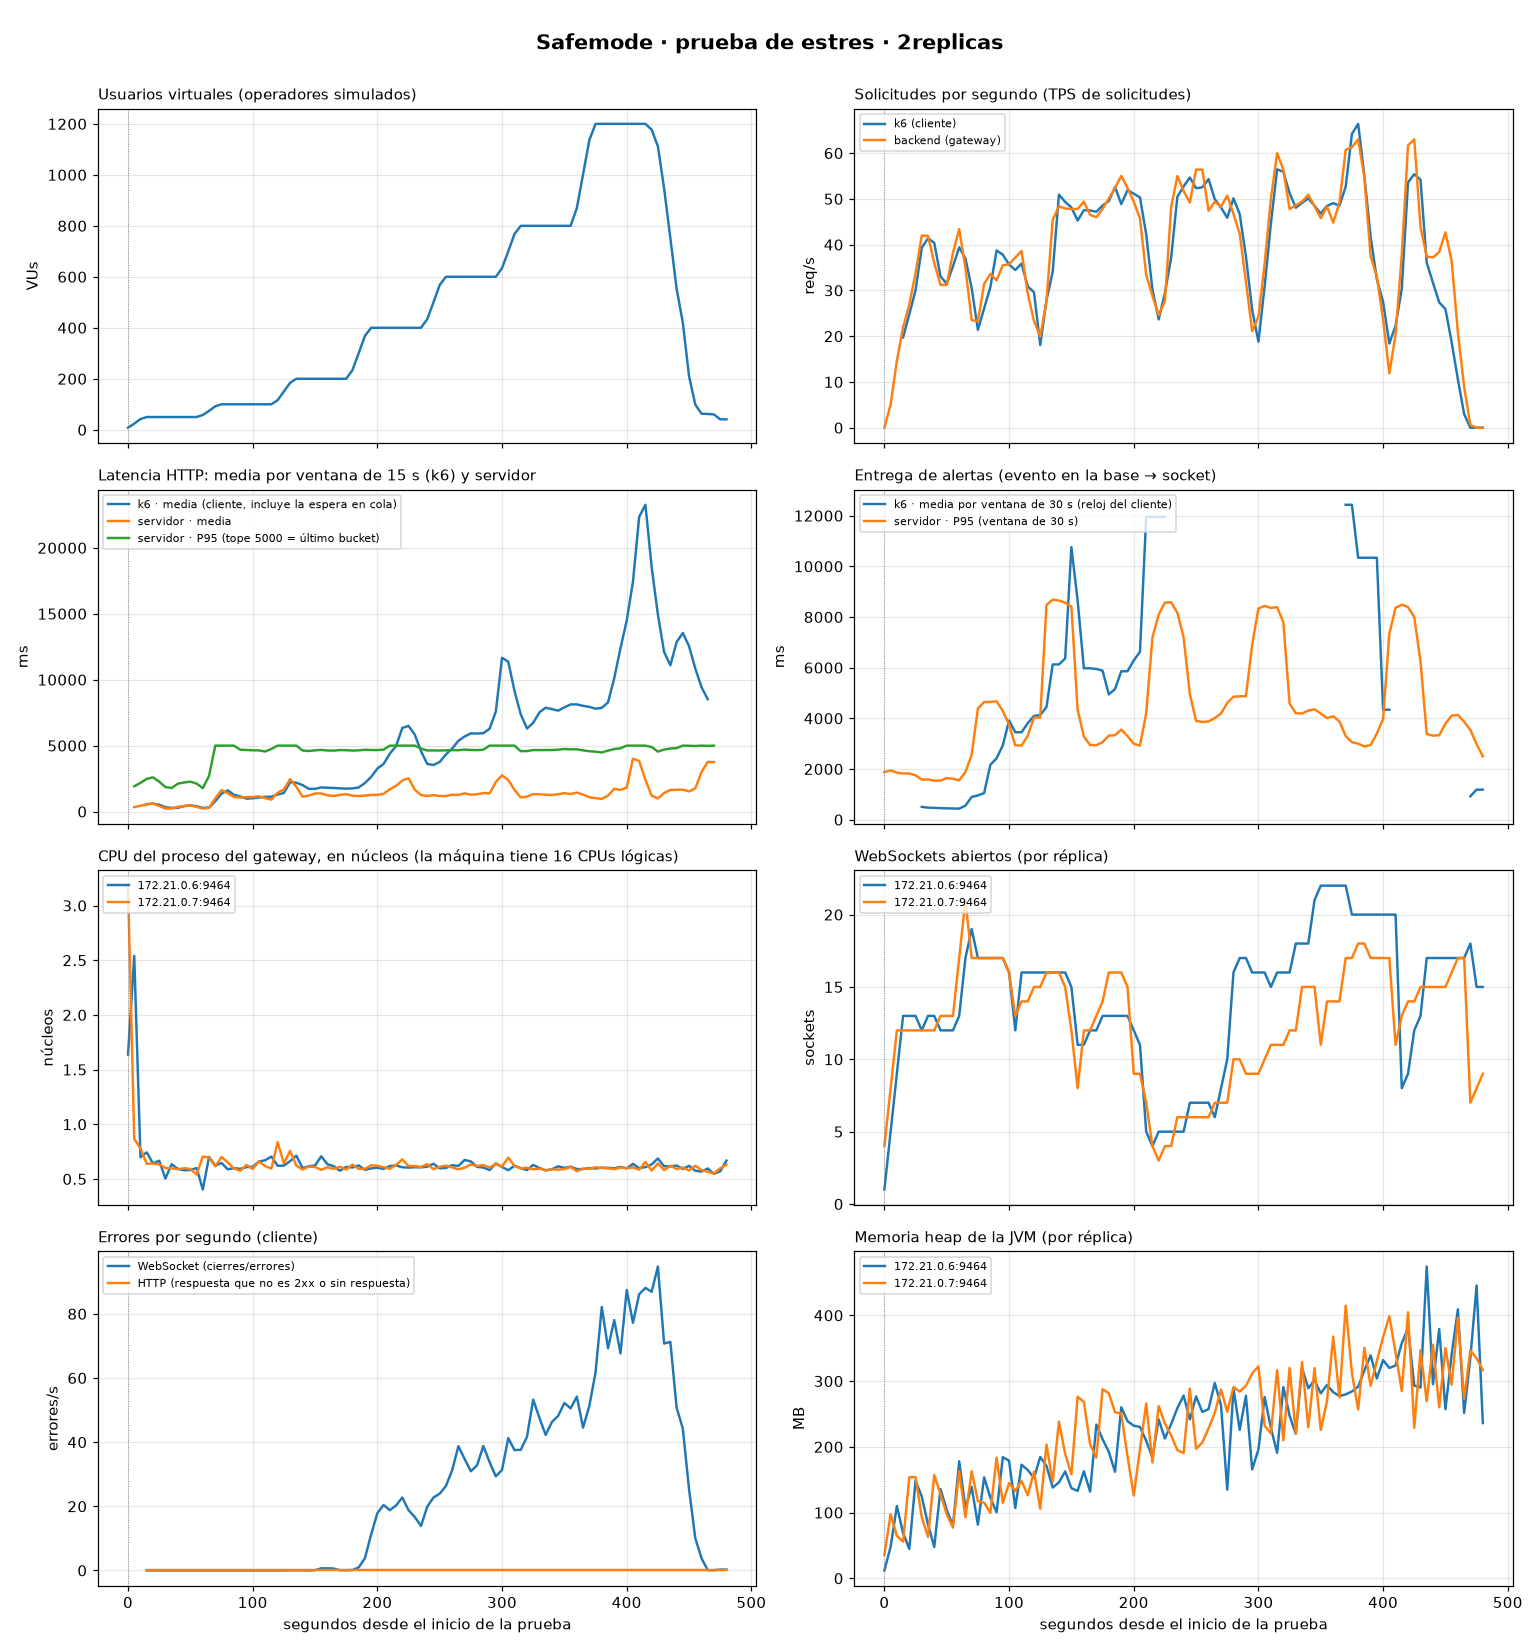
\includegraphics[width=0.96\textwidth,height=0.85\textheight,keepaspectratio]{../rendimiento/resultados/estres-2replicas/estres-2replicas.png}
\caption{Estrés con 2 réplicas \emph{antes} de la corrección: el TPS se aplana en torno a 40 req/s, la media del servidor se queda en 1~s y la del
cliente crece; la CPU del gateway no pasa de 0,7 núcleos.}\label{fig:estres-antes}
\end{figure}

\begin{figure}[p]
\centering
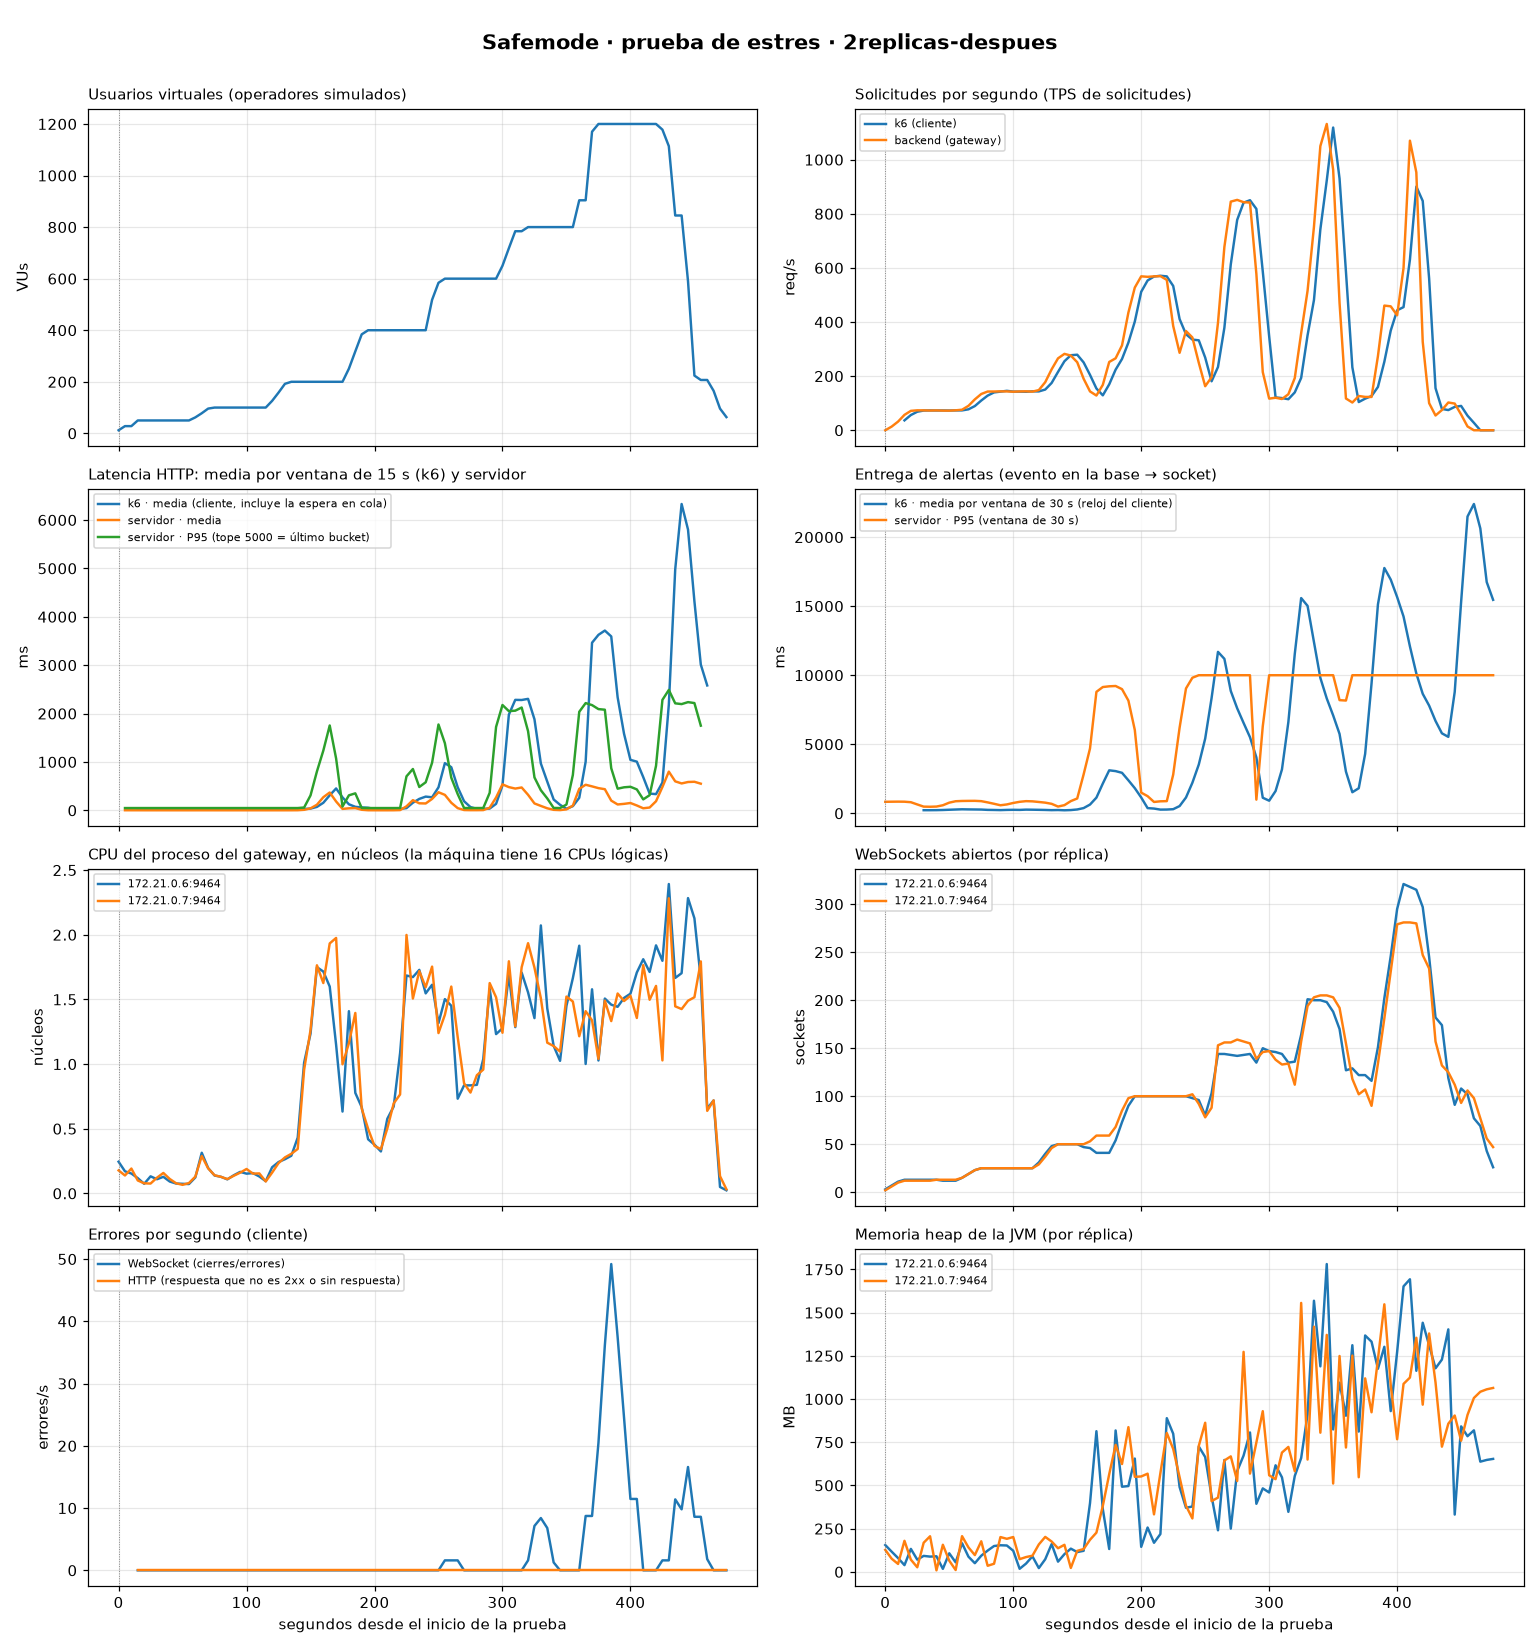
\includegraphics[width=0.96\textwidth,height=0.85\textheight,keepaspectratio]{../rendimiento/resultados/estres-2replicas-despues/estres-2replicas-despues.png}
\caption{Estrés con 2 réplicas \emph{después} de la corrección: HTTP llega a 678 req/s por escalón (picos de 1\,119 req/s), sin errores HTTP;
la entrega de alertas pasa a ser el límite.}\label{fig:estres-despues}
\end{figure}

% ------------------------------------------------------------------------------------------------------------------------------------
\section{Escalabilidad y disponibilidad}\label{sec:disponibilidad}

\begin{table}[H]
\centering\small
\caption{Escenario de disponibilidad y escalabilidad ED-1.}\label{tab:ed1}
\begin{tabularx}{\textwidth}{lY}
\toprule
\textbf{Fuente} & Un fallo interno: una réplica del gateway termina (error, falta de memoria o despliegue de una versión nueva) \\
\textbf{Estímulo} & Con operadores conectados y alertas llegando, una réplica deja de responder de golpe (SIGKILL) o termina sola \\
\textbf{Artefacto} & Capa de gateway (HTTP, WebSocket y motor de alertas) detrás del balanceador, con la base compartida \\
\textbf{Entorno} & Operación normal con carga continua y varios operadores con el panel abierto \\
\textbf{Respuesta} & El balanceador la excluye (vigilancia activa de \cod{/ready} y pasiva por conexión rechazada) y reintenta en la otra; los operadores se reconectan solos con la misma sesión; una alerta creada durante la caída llega a todos; la réplica se reinicia y vuelve \\
\textbf{Medida} & 0 peticiones fallidas; reconexión $\leq$ 2,1~s; 0 alertas perdidas o duplicadas; réplica de nuevo en rotación en $\approx$ 5~s \\
\bottomrule
\end{tabularx}
\end{table}

\textbf{Tácticas} \cite{bass}: detectar fallos (ping/echo sobre \cod{/ready}, que comprueba la base); recuperarse (redundancia activa de dos réplicas,
reintento, reinicio automático con \cod{restart: unless-stopped}); prevenir fallos (eliminar el estado local: las sesiones y las alertas viven
en la base, y cada réplica reconstruye lo que le falta).

\textbf{Qué se cambió en el código para poder escalar} (ADR~0006): (1) las alertas llegan a todas las réplicas porque cada una sondea la tabla
cada 0,5~s; (2) la creación de una alerta resiste la carrera entre réplicas (el \cod{UNIQUE} de la base decide y el SQLState 23505 se trata como
«ya existe»); y (3) las sesiones pueden guardarse en la base (\cod{SAFEMODE_SESSION_STORE=database}, con la huella SHA-256 del identificador y
falla cerrada), de modo que cualquier réplica reconoce la cookie que emitió otra.

\textbf{Cálculo de disponibilidad con los SLA publicados por AWS.} Hoy el despliegue público es un solo servidor y su disponibilidad es la de
una instancia EC2 (99,5\,\%, unas 3,6~h de caída al mes). El diseño objetivo (DNS $\rightarrow$ balanceador multi-AZ $\rightarrow$ dos gateways en
dos zonas $\rightarrow$ RDS Multi-AZ) llega a \textbf{99,9375\,\%} (3,2 «nueves», 27~min al mes), con la base de datos pesando el 80\,\% de la
indisponibilidad restante. Dos réplicas en el mismo servidor no mejoran nada: comparten instancia, zona y disco.

\begin{table}[H]
\centering\small
\caption{Prototipo de dos réplicas (tres corridas, 17/17 comprobaciones cada una; docs/disponibilidad/).}\label{tab:escalado}
\begin{tabularx}{\textwidth}{lY}
\toprule
\textbf{Medida} & \textbf{Resultado} \\
\midrule
Reparto de 30 peticiones con una sola sesión & 15 y 15 entre las réplicas; 30 de 30 con 200 \\
Caída de golpe (SIGKILL) con tráfico & \textbf{0 de 555 peticiones fallaron}; p50 45~ms, p99 250~ms \\
Reconexión de los operadores de la réplica caída & 2,07~s el más lento (2~s son la espera del panel) \\
Alerta creada durante la caída & 3 la recibieron en vivo y 3 al reconectar; ninguna perdida ni duplicada \\
Réplica de nuevo en rotación & 5,2~s si Docker la reinicia; 8,3~s si se arranca a mano \\
\bottomrule
\end{tabularx}
\end{table}

\textbf{Límite honesto.} 0 fallos en 555 peticiones solo permite afirmar, con 95\,\% de confianza, una disponibilidad de al menos 99,46\,\%
(regla de los tres): el prototipo mide el \emph{comportamiento ante fallos}, no la disponibilidad de largo plazo. Y el despliegue público sigue
siendo un servidor único: el despliegue distribuido en dos zonas está diseñado y calculado (Figura~\ref{fig:despliegue-objetivo}) pero no
desplegado, porque requiere recursos de AWS y una decisión de costo del equipo.

% ------------------------------------------------------------------------------------------------------------------------------------
\section{Seguridad}\label{sec:seguridad-resumen}
Tres escenarios, \textbf{aprobados por el docente}, con tácticas y validación ejecutable (capítulo~\ref{chap:seguridad}):
ES-1 autenticación y autorización del operador (35 pruebas), ES-2 protección frente a ataques web y revocación de sesión, y ES-3 integridad del
canal de imágenes \cod{/frames} (12 comprobaciones reproducibles). La sesión es una cookie de 256 bits \cod{HttpOnly} y \cod{SameSite=Strict}
de 12~h; el servidor guarda solo su huella SHA-256 y toda ruta protegida responde 401 sin sesión antes de ejecutar su manejador.

% ------------------------------------------------------------------------------------------------------------------------------------
\section{Portabilidad}\label{sec:portabilidad}

\begin{table}[H]
\centering\small
\caption{Escenario de portabilidad PT-1 (migración Cloud $\rightarrow$ On-Premise).}\label{tab:pt1}
\begin{tabularx}{\textwidth}{lY}
\toprule
\textbf{Fuente} & El equipo (o un cliente) que debe mover SafeMode de AWS a servidores propios \\
\textbf{Estímulo} & Decisión de migrar: no hay instancias EC2 ni servicios administrados de AWS disponibles \\
\textbf{Artefacto} & Todos los componentes: gateway, tracker, servicios de acceso y colaboración, bases de datos, proxy y observabilidad \\
\textbf{Entorno} & Un servidor Linux con Docker y Docker Compose, red local y dominio propio \\
\textbf{Respuesta} & Se clona el repositorio, se copia \cod{.env.example} a \cod{.env} con los valores propios y se levanta el mismo Compose; no hay cambios de código \\
\textbf{Medida} & 0 líneas de código cambiadas; todo componente se ejecuta en un contenedor o con una sola orden; la configuración sale solo de variables de entorno \\
\bottomrule
\end{tabularx}
\end{table}

\textbf{Evidencia.} Los componentes se empaquetan en contenedores (\cod{Dockerfile} por servicio) y el mismo conjunto de archivos Compose se
usa en tres entornos: el computador del desarrollador (Windows con Docker Desktop, donde corrieron todas las pruebas de este documento), el
prototipo de escalado y el servidor de AWS (\cod{docker-compose.publico.yml} con Caddy). La capa de datos se eligió sin dependencias de
proveedor: PostgreSQL, MongoDB y Redis en contenedores, y H2 como valor por defecto sin base externa; la única pieza propia de AWS es la
instancia que ejecuta Docker. El DNS (DuckDNS) y los certificados (Let's Encrypt, que gestiona Caddy) tampoco son de AWS. La guía
\cod{docs/despliegue/} y el script \cod{verificar-despliegue.ps1} comprueban el sitio publicado con peticiones de solo lectura.

\textbf{Qué cambiaría al migrar.} Solo lo operativo: el dominio y su DNS, la ruta del volumen de fotos, la rotación de claves y, si se
quiere alta disponibilidad, el balanceador (Caddy ya cumple ese papel en el prototipo) y la base replicada. \textbf{Límite declarado:} la
migración a un servidor on-premise distinto del equipo de desarrollo no se ejecutó como prueba; lo que se valida es que el mismo stack ya corre
en dos entornos distintos sin cambios.

% ------------------------------------------------------------------------------------------------------------------------------------
\section{Mantenibilidad}\label{sec:mantenibilidad}

\begin{table}[H]
\centering\small
\caption{Escenario de mantenibilidad MT-1 (inspección continua con análisis estático).}\label{tab:mt1}
\begin{tabularx}{\textwidth}{lY}
\toprule
\textbf{Fuente} & Una persona del equipo que sube un cambio al repositorio \\
\textbf{Estímulo} & \cod{git push} a cualquier rama o ejecución manual del workflow \\
\textbf{Artefacto} & Código fuente: backend Java (8 módulos Maven) y panel en JavaScript \\
\textbf{Entorno} & Integración continua en GitHub Actions, antes de cualquier despliegue \\
\textbf{Respuesta} & Compila, ejecuta las pruebas, mide la cobertura de cada capa y analiza estáticamente; si el control de calidad falla, el job falla y el despliegue no corre \\
\textbf{Medida} & Cobertura $\geq$ 80\,\% en backend y panel; fiabilidad, seguridad y mantenibilidad en A; control de calidad en verde \\
\bottomrule
\end{tabularx}
\end{table}

\textbf{Pipeline con reusable workflows.} \cod{pipeline.yml} llama a \cod{reusable-backend.yml} (\cod{mvn verify} con JaCoCo),
\cod{reusable-frontend.yml} (pruebas del panel con c8) y \cod{reusable-sonar.yml} (análisis con control de calidad), y el despliegue de la
EC2 depende de la calidad. La cobertura que se reporta es la de las pruebas que se ejecutan en esa corrida, no un número escrito a mano.

\begin{table}[H]
\centering\small
\caption{Resultados medidos (backend con JaCoCo; panel con c8; calificaciones con SonarQube Community 26.11 local).}\label{tab:mt-resultados}
\begin{tabularx}{\textwidth}{lYY}
\toprule
\textbf{Medida} & \textbf{Resultado} & \textbf{Meta} \\
\midrule
Cobertura de líneas del backend (479 pruebas) & 81,8\,\% (núcleo del producto 91,6\,\%) & $\geq$ 80\,\% \\
Cobertura del panel (144 pruebas, \cod{--all}) & 99,3\,\% de líneas & $\geq$ 80\,\% \\
Fiabilidad, seguridad, mantenibilidad & A, A, A (0 errores, 0 vulnerabilidades) & A \\
Control de calidad de Sonar & Verde; cobertura del código nuevo 98,5\,\% & Verde \\
Duplicación; olores de código & 0\,\%; 1 (no afecta calificación) & --- \\
\bottomrule
\end{tabularx}
\end{table}

\textbf{Lo que el análisis encontró.} Antes de la primera calificación había 4 errores y 4 «vulnerabilidades». Cuatro errores eran reales
(registros con arreglos que comparaban identidad, una expresión regular ambigua y un campo sin etiqueta) y se corrigieron con prueba. Las
cuatro «vulnerabilidades» de SQL formateado eran falsos positivos (solo reciben constantes del dialecto) y quedaron justificadas en el código.
Medir la cobertura del panel (41\,\% $\rightarrow$ 99\,\%) destapó además dos defectos reales de la interfaz. \textbf{Límites:} el script en
línea de \cod{index.html} no está medido; la corrida real en SonarCloud requiere la cuenta del equipo; y los adaptadores a bases de datos
(PostgreSQL, MongoDB, Redis) se prueban contra las bases reales fuera del pipeline.

% ------------------------------------------------------------------------------------------------------------------------------------
\section{Observabilidad}\label{sec:observabilidad}

\begin{table}[H]
\centering\small
\caption{Escenario de observabilidad OB-1.}\label{tab:ob1}
\begin{tabularx}{\textwidth}{lY}
\toprule
\textbf{Fuente} & Un operador del sistema (o el docente) que necesita saber si SafeMode funciona y por qué se degrada \\
\textbf{Estímulo} & Una dependencia cae (PostgreSQL, Redis, el servicio de acceso) o la latencia sube bajo carga \\
\textbf{Artefacto} & Métricas de aplicación y de dependencias; Prometheus; Grafana; reglas de alerta \\
\textbf{Respuesta} & El tablero muestra tráfico, latencia, errores, CPU, memoria y estado de cada dependencia; una regla de Prometheus se dispara y dice qué hacer \\
\textbf{Medida} & La degradación se detecta en $\leq$ 1~min (\cod{for: 1m}); cada dependencia publica \cod{safemode_dependency_up} (1 sirve, 0 cae) \\
\bottomrule
\end{tabularx}
\end{table}

\textbf{Qué se instrumentó.} El gateway publica métricas con Micrometer en el puerto 9464 (tráfico, latencia y errores por ruta
\cod{safemode_http_request_seconds}, entrega de alertas \cod{safemode_alert_delivery_seconds}, sockets abiertos, alertas por severidad y tipo, y
el estado de la base como dependencia); los servicios de acceso y colaboración publican las suyas. Prometheus recoge cada réplica por DNS, y Grafana
muestra el tablero del equipo (\cod{observability/dashboards/dashboard-safemode-v2.json}) junto con los de persistencia. k6 envía sus métricas a
Prometheus por \emph{remote write}, de modo que las pruebas de carga se ven en el mismo tablero antes, durante y después.

\textbf{Condiciones de degradación detectables.} Ocho reglas (\cod{performance/monitoring/reglas-alertas.yml}, validadas con \cod{promtool}):
gateway caído, base inaccesible, réplica no lista, latencia HTTP alta, entrega de alertas lenta, errores 5xx, CPU alta y demasiados sockets. En las
pruebas se dispararon las de \textbf{latencia} y de \textbf{entrega}; la de CPU no, porque el cuello de botella no era la CPU: una enseñanza
útil, pues vigilar solo el recurso habría dado una falsa tranquilidad. \textbf{Pendiente:} la captura del tablero con el período de una prueba.

% ------------------------------------------------------------------------------------------------------------------------------------
\section{Robustez en concurrencia y tiempo real}\label{sec:concurrencia}

\begin{table}[H]
\centering\small
\caption{Escenario de concurrencia CO-1 (laboratorio de consistencia, ADR~0005).}\label{tab:co1}
\begin{tabularx}{\textwidth}{lY}
\toprule
\textbf{Fuente} & Dos operadores que editan a la vez la configuración del puesto; una dependencia que cae a mitad de una operación \\
\textbf{Estímulo} & Dos escrituras con la misma versión; una revocación de permiso; Redis o el servicio de acceso detenidos \\
\textbf{Respuesta} & Una escritura gana (200) y la otra recibe 409; se rechaza la escritura de quien perdió el permiso (403); si no se puede verificar el permiso, no se guarda (503) \\
\textbf{Medida} & Antes: dos 200 y una edición perdida; después: [200, 409] y revocado 403 con el documento intacto; 4 de 4 comprobaciones \\
\bottomrule
\end{tabularx}
\end{table}

\textbf{Mecanismos.} La versión viaja \emph{en el filtro} de la misma operación atómica de MongoDB (\cod{findOneAndUpdate}), de modo que no hay
ventana entre leer y escribir; el permiso se pregunta siempre a la autoridad (PostgreSQL) y la caché de Redis solo sirve para pintar la
pantalla, nunca para autorizar; la presencia y el permiso en caché se guardan con su vencimiento en una sola escritura (\cod{SET ... EX}).
En el producto, una alerta es única por evento aunque haya varios paneles o réplicas (\cod{UNIQUE} en la base), y dos cámaras se analizan en
paralelo con un seguimiento independiente por cámara. \textbf{Límite declarado:} PostgreSQL y MongoDB no comparten transacción, por lo que
entre validar el permiso y guardar queda una ventana pequeña; la alternativa (PostgreSQL con JSONB) está explicada en el ADR.
